\documentclass[varwidth=true, border=2pt]{standalone}

\usepackage{pgfplots}
\usepackage{tikz}

\begin{document}
	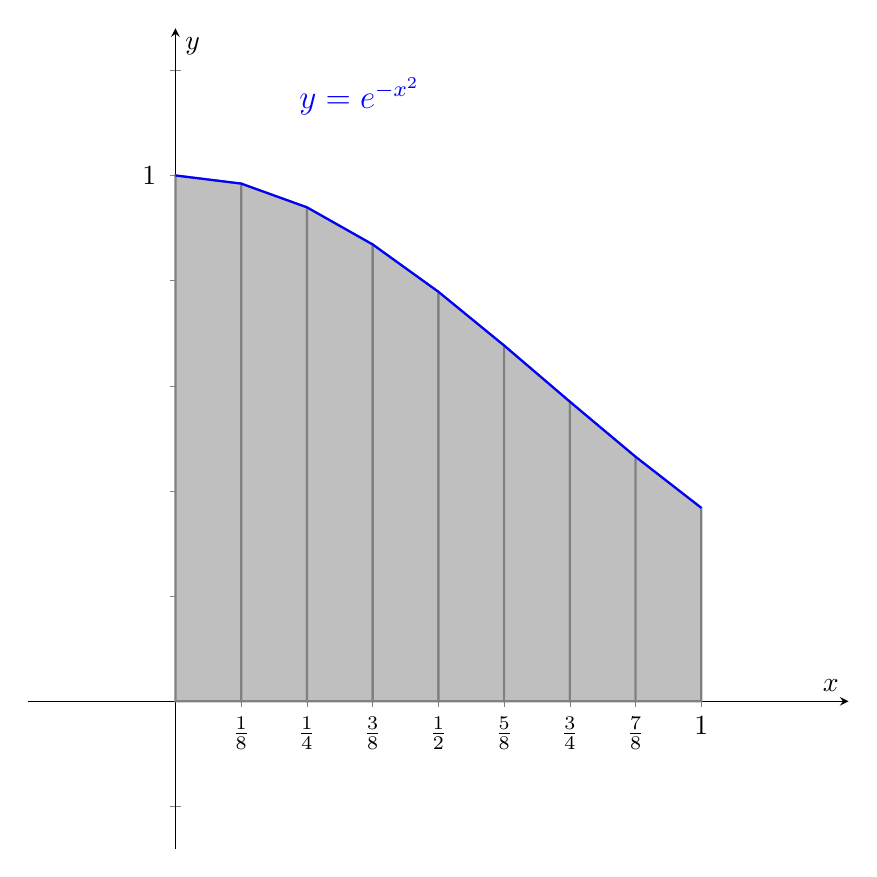
\begin{tikzpicture}
    \begin{axis}[
    xtick={0.125,0.25,...,1 },
        legend pos=south east,
        axis x line=middle,
        axis y line=middle,
	xticklabels={$\frac{1}{8}$, $\frac{1}{4}$,$\frac{3}{8}$,$\frac{1}{2}$,$\frac{5}{8}$,$\frac{3}{4}$,$\frac{7}{8}$,$1$},
	yticklabels= \empty,
        grid = none ,
        width=12cm,
        height=12cm,
        grid style={dashed, gray!1},
        xmin=-0.15,     % start the diagram at this x-coordinate
        xmax=1.15,    % end   the diagram at this x-coordinate
        ymin=-0.15,     % start the diagram at this y-coordinate
        ymax= 1.15,   % end   the diagram at this y-coordinate
        xlabel=$x$,
        ylabel=$y$,
        enlargelimits=true,
        tension=0.08]
        
        \node(A1) at (axis cs: 0, 0){};
        \node(A2) at (axis cs: 0,1){};
       \node(B1) at (axis cs: 0.125, 0){};        
        \node(B2) at (axis cs: 0.125, 0.9845){};
         \node(C1) at (axis cs: 0.25,0){};
         \node(C2) at (axis cs: 0.25,0.9394){};
         \node(D1) at (axis cs: 0.375,0){};
         \node(D2) at (axis cs: 0.375,0.8688){};
         \node(E1) at (axis cs: 0.5,0){};
         \node(E2) at (axis cs: 0.5,0.7788){};
         \node(F1) at (axis cs: 0.625,0){};
         \node(F2) at (axis cs: 0.625,0.6766){};
         \node(G1) at (axis cs: 0.75,0){};
         \node(G2) at (axis cs: 0.75,0.5698){};
         \node(H1) at (axis cs: 0.875,0){};
         \node(H2) at (axis cs: 0.875,0.4650){};
         \node(I1) at (axis cs: 1,0){};
         \node(I2) at (axis cs: 1,0.3678){};


\draw[draw = gray, thick,  fill = lightgray] (A1.center) -- (A2.center) -- (B2.center) -- (B1.center) -- cycle;
\draw[draw = gray, thick,  fill = lightgray] (B1.center) -- (B2.center) -- (C2.center) -- (C1.center) -- cycle;
\draw[draw = gray, thick,  fill = lightgray] (C1.center) -- (C2.center) -- (D2.center) -- (D1.center) -- cycle;
\draw[draw = gray, thick,  fill = lightgray] (D1.center) -- (D2.center) -- (E2.center) -- (E1.center) -- cycle;
\draw[draw = gray, thick,  fill = lightgray] (E1.center) -- (E2.center) -- (F2.center) -- (F1.center) -- cycle;
\draw[draw = gray, thick,  fill = lightgray] (F1.center) -- (F2.center) -- (G2.center) -- (G1.center) -- cycle;
\draw[draw = gray, thick,  fill = lightgray] (G1.center) -- (G2.center) -- (H2.center) -- (H1.center) -- cycle;
\draw[draw = gray, thick,  fill = lightgray] (H1.center) -- (H2.center) -- (I2.center) -- (I1.center) -- cycle;
\draw[draw = blue, thick] (A2.center) -- (B2.center) -- (C2.center) -- (D2.center) -- (E2.center) -- (F2.center) -- (G2.center) -- (H2.center) -- (I2.center);

  




	\node(a) at (axis cs: -0.05,1){1};
	\node(MP)[blue] at (axis cs: 0.35,1.15){\large{$y=e^{-x^2}$}};
    \end{axis}
\end{tikzpicture}
\end{document}